\chapter{FM-радио для хипстера}

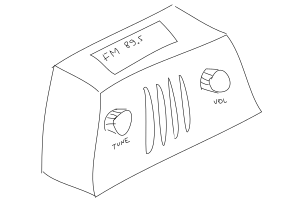
\includegraphics{sketches/fm-radio}

Итак, наконец-то, к первому проекту! Начнём с чего-нибудь простого, но в то же время условно-полезного. В качестве такого устройства я выбрал настольное FM-радио с классическим управлением двумя поворотными ручками и ЖК-дисплеем для отображения информации.

Вроде бы уже давно настала эра цифрового радио и стриминг-сервисов, но всё равно, порой не хватает аскетичного приёмника, который можно включить одним движением без поиска нужной иконки, без сопряжения с беспроводными колонками, без всей этой суеты. А с учётом того, что вы можете сделать уникальный корпус, можно быть уверенным, что самоделка займёт своё место в интерьере. Поехали!

% TODO: перечислить фактические знания

В этой главе вы узнаете, как работать с текстовым ЖК-экраном, энкодером и чипом FM-приёмника; что такое шина I²C; как устроено воспроизведение звука; и многое другое.

\section{Необходимое железо}

% TODO: лист картинок

\begin{itemize}
  \item Ардуино-совместимая плата: Arduino Uno, Iskra Uno, Iskra Nano или другая
  \item USB-кабель для прошивки и питания
  \item Модуль FM-приёмника на чипе TEA5767
  \item Усилитель аудиосигнала, например, на основе микросхемы PAM8403
  \item Динамик с импедансом 4 или 8 Ом
  \item Потенциометр для управления громкостью
  \item Поворотный энкодер для переключения радиостанций
  \item Текстовый ЖК-экран
  \item Провода
  \item Беспаечная макетка (breadboard) для прототипа
\end{itemize}

Опционально:

\begin{itemize}
  \item Модуль пауэр-банк для автономной работы
  \item Тумблер для включения / выключения
  \item Макетка под пайку для финальной сборки
  \item Гнездо под штекер 3.5 мм с клеммником
\end{itemize}

\section{Как вещает радио}

Вы конечно знаете, что эфир радиостанций распространяется по-воздуху в виде неких магических невидимых волн. Где-то на радиостанции стоят антенны и оборудование, которые перепаковывают звуковой сигнал в электромагнитный и вещают его во все стороны. Если мы хотим услышать, что происходит в эфире, мы должны этот радиосигнал поймать, распаковать обратно в звуковой вид и отправить на динамик.

Но как это сделать? Нужно разобраться, как устроен FM-сигнал. Итак, по воздуху можно распространять радиоволны. У каждой радиоволны есть \emph{частота}. Эта характеристика говорит о том, сколько раз в секунду встречается пик этой волны. Например, частота в 89.5 мегагерц означает, что пик будет встречаться 89.5 миллионов раз в секунду. Часто, не правда
ли? Волны разной частоты можно отделять друг от друга, немного корректируя схему приёмника. Поэтому, на частоте 89.5 МГц сигнал может транслировать одна радиостанция, а на частоте 90.0 Мгц уже другая. При этом они не будут мешать вашему домашнему Wi-Fi, потому что он вовсе работает на частоте около 2.4 или 5 ГГц.

\begin{figure}
  \centering
  % TODO: перерисовать через Matplotlib + xkcd, показать суперпозицию
  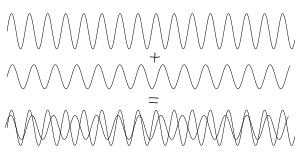
\includegraphics{sketches/wave-lengths}
  \caption{Волны разной частоты формируют эфир}
\end{figure}

\begin{Note}
  А вот сигналы, посылаемые волнами схожих частот очень даже мешают друг
  другу и это серьёзная проблема современных городов, которая заставляет
  занимать для разных целей всё новые и новые диапазоны частот. Диапазон
  частот называется полосой, а разрешают или запрещают их использование
  разные дядьки в министерствах. Но это уже другая история.
\end{Note}

Хорошо, с частотой несущей волны разобрались. Но как с помощью неё передать информацию? В нашем случае звуковой ряд. Тут в дело вступает трюк, который называется модуляцией. Кстати, «FM» означает «фазовая модуляция». Суть трюка заключается в том, чтобы менять фазу несущей частоты в соответствии с тем, какой звуковой сигнал нужно передать: несущую волну сжимают и растягивают как гармошку, чтобы дополнить полезной информацией. Драматично на частоту несущей волны это не влияет, т.к. силы не равны: килогерцы звуковой волны против гигагерц несущей.

% TODO "Грубая иллюстрация принципа фазовой модуляции"
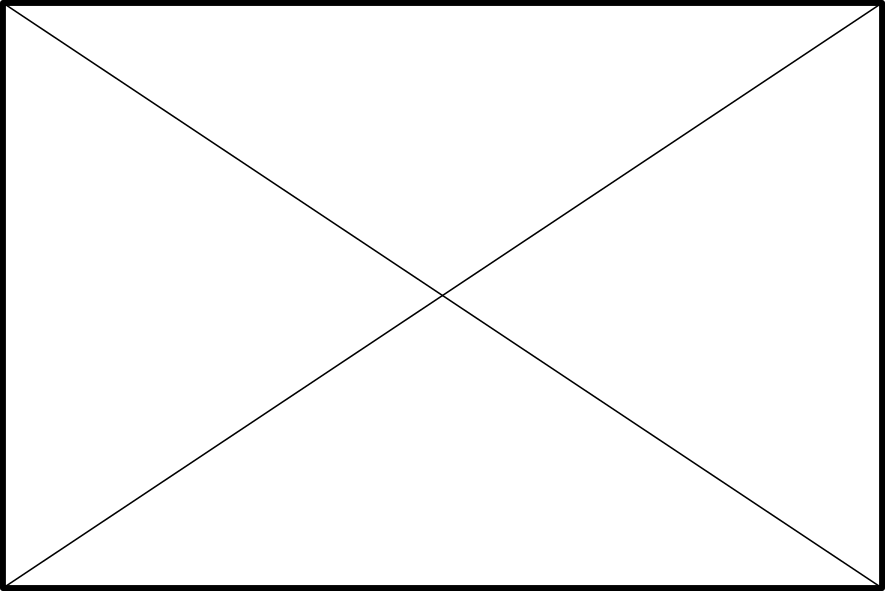
\includegraphics{TODO.png}

Вроде бы разобрались. Так как имея на руках несколько проводов и пару резисторов, поймать волну и расшифровать её? Можно собрать внушительную схему из отдельных компонентов, как делали наши отцы и деды. Но время идёт и для многих типовых задач давно существуют готовые \emph{микросхемы} (также известные как \emph{чипы}), которые скрывают всю схему под крохотным пластиковым корпусом, а для своей работы требуют минимум дополнить компонентов.

\section{Знакомьтесь, TEA5767!}

Чипом, предназначенным специально для приёма и демодуляции FM-радио является дешёвый и популярный TEA5767 от компании Philips. В своём оригинальном виде он предназначен для ширпотребной и миниатюрной электроники, которую производят промышленным образом. Поэтому он настолько мал, что вам, как мейкеру, было бы крайне неудобно работать с ним, если речь идёт о ручной сборке одного или нескольких устройств. К тому же для своей работы он требует несколько дополнителльных компонентов вроде кварцевого резонатора.

Ленивое и алчное человечество не остановилось на создании миниатюрных чипов. Специально для вас, мейкеры, некоторые компании берут такие маленькие чипы, увеличивают их в размерах, распаивая на печатной плате вместе с необходимым обвесом и продают втридорога \textbar emoji\_smiling\_imp\textbar{} Но ведь девайс собранный своими руками бесценен, не так ли?!

Для нашего радио нам понадобится один из таких готовых модулей.

\begin{figure}
  \centering
  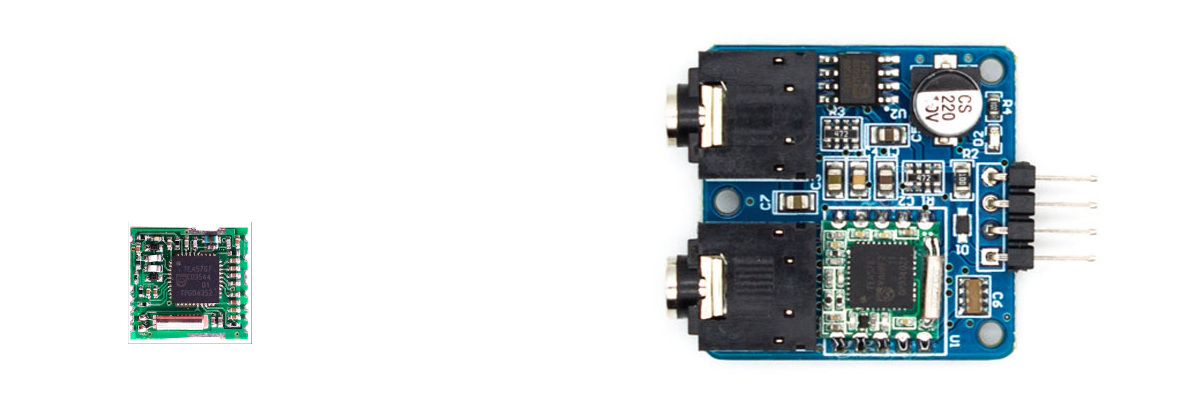
\includegraphics{TEA5767.jpg}
  \caption{Популярные вариации модуля на базе TEA5767}
\end{figure}

Что же он из себя представляет? Такой модуль является безголовым радио, которым нужно управлять не кнопками и ручками, как на готовой аудио-системе, а командами с конроллера. Контроллером может запросто выступать ваша Arduino-совместимая плата. Контроллер может попросить настроиться на определённую частоту, начать промотку каналов в одну или другую сторону, запросить уровень сигнала, а в качестве выхода модуль на TEA5767 выдаёт аудиосигнал.

\begin{figure}
  \centering
  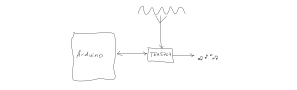
\includegraphics{sketches/fm-receiver-diagram}
  \caption{Диаграмма включения модуля FM-приёмника}
\end{figure}

Давайте теперь разберёмся, как именно общаться с модулем. Такой модуль с точки зрения взаймодействия несколько сложнее, чем светодиод или кнопка: коммуникация с ним строится через так называемый интерфейс I²C. Пусть вас это не пугает: благодаря тому, что для популярных модулей уже созданы библиотеки, работа с ними становится вполне тривиальной.

\begin{Note}
  % TODO: emoji
  Я надеюсь, что вы не сильно устали, потому что всё написанное выше и под следующим заголовком на деле не нужно для того, чтобы сделать радио \textbar emoji\_smile\textbar. Но этими знаниями можно вполне хвастануть за бокалом пива. Сразу после, обещаю, мы приступим к сборке.
\end{Note}

\section{Интерфейс I²C}

I²C, он же IIC, он же «айтуси», он же «идвацэ», он же TWI — крайне распространённый интерфейс в мире цифровой микроэлектроники для подключения устройств. Так если в своём компьютере вы скорее всего найдёте интерфейсы USB, Display Port и Ethernet, то на конроллере вы найдёте другой набор интерфейсов: UART, SPI и I²C. Они пусть менее гибкие и богатые на возможности, но гораздо более простые и непритязательные к вычислительным ресурсам.

В случае с I²C всегда одно из устройств выступает ведущим (master), а другое ведомым (slave). Ведущим как правило является контроллер Arduino, а ведомым — модуль или чип. Обмен данными между устройствами по I²C осуществляется по двум сигнальным линиям, т.е. проводам:

% TODO: definition list

SDA Линия данных. Высокий сигнал вроде 3.3 или 5 вольт (зависит от родного напряжения участников) означает передачу бита-единички, низкий сигнал 0 вольт означает передачу бита-нолика. В какую сторону передаются данные в данный конкретный момент зависит от ситуации, а вернее от \emph{протокола}, на который негласно договорились участники коммуникации.

SCL Линия тактирования. Очередной бит считается переданным, после того как линия сначала получает высокий сигнал, а затем низкий. Сигналом на SCL всегда управляет мастер, вне зависимости от направления передачи данных. Так он задаёт скорость коммуникации. Задача ведомого устройства — поспевать.

\begin{figure}
  \centering
  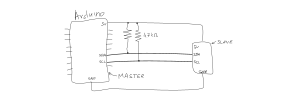
\includegraphics{sketches/i2c-single}
  \caption{Типовой пример подключения одного I²C-устройства}
\end{figure}

I²C — это шина (bus). Под этим понимается, что на одной и той же паре линий SDA/SCL может быть подключено множество разных устройств. Если быть точным, до 127 ведомых устройств.\footnote{Если быть совсем точным, то расширенный стандарт позволяет подключить в теории и до 32 тысяч устройств, но это совсем экзотика. В мире хобби-электроники не встречал.} При этом, у любого устройства на шине, будь оно единственным или нет, есть собственный адрес, по которому ведущий обращается именно к нему.

\begin{figure}
  \centering
  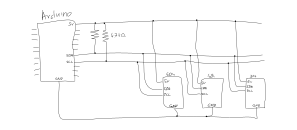
\includegraphics{sketches/i2c-multiple}
  \caption{Типовой пример подключения нескольких I²C-устройств}
\end{figure}

С этой точки зрения, шина I²C похожа на роту модулей построенную на плацу, где командование ведёт офицер-контроллер. Все слышат всё, но говорит только один:

— Рядовой 60h!\\
— Здесь!\\
— Частоту радио на 89.5 МГц установить!\\
— Есть!\\
— Частоту радио на 1000 МГц установить!\\
— Никак нет!\\
— Уровень сигнала сообщить!\\
— Двенадцать!

Адрес конкретного модуля обычно жёстко задаётся на производстве, на уровне микросхемы. Например, адрес TEA5767 — 60 в шестнадцатиричной системе, что обычно записывают как \texttt{60h} или \texttt{0x60}.  Детали протокола также определяются разработчиками модуля, а все его подробности всегда подробно описаны в даташите от производителя.

К счастью, для многих популярных модулей уже существуют высокоуровневые библиотеки-обёртки, которые вовсе снимают необходимость в том, чтобы разбираться в тонкостях их протоколов. Это справедливо и для нашего FM-приёмника. Так что мы уже готовы действовать. Вперёд!

\section{Подключаем модуль FM-приёмника}

% TODO: ref

Будем строить девайс в несколько этапов. Сначала попробуем заставить выдавать наше радио хоть что-то. Для этого соберите схему, как показано на рисунке :numref:fig\emph{fm-radio}wire-tea5767.

\begin{figure}
  \centering
  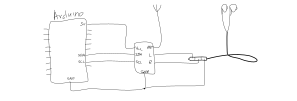
\includegraphics{sketches/tea5767-wiring}
  \caption{Схема подключения модуля TEA5767 к Arduino}
\end{figure}

Для сборки используйте макетные провода и бредборд. Где возможно, не соединяйте пока всё намертво паяльником: нам ещё предстоит дополнять схему. И в конце концов, нужно предварительно убедиться, что всё работает.

% TODO: ref

В зависимости от выбранной модели FM-модуля вам может понадобиться припаять к модулю ножки-штырьки. Если на борту модуля нет разъёма 3.5 мм для непосредственного подключения наушников, вы можете использовать TRS-гнездо с клеммником, чтобы быстро адаптировать пины L, R и GND на модуле в стандартный аудиоразъём (:numref:fig\emph{fm-radio}trs-socket).

\begin{figure}
  \centering
  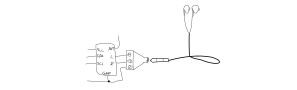
\includegraphics{sketches/trs-35-mm}
  \caption{Подключение наушников через клеммный разъём 3.5 мм}
\end{figure}

А нельзя ли сразу подключить динамик, который мы планируем использовать в финальном устройстве? Нет, пока нет. Дело в том, что модуль выдаёт слишком слабый аудиосигнал, который не сможет качать мембрану крупного динамика. Но на маленькие наушники его вполне хватит. Подойдёт также колонка с активным усилением, то есть та, у которой есть собственное питание и регулировка громкости.

В качестве антенны можно использовать ту, что была в комплекте с модулем, если она была, но в любом случае с этой задачей отлично справится простой кусок провода. Это даже лучше с эстетической точки зрения: его можно будет смотать и спрятать внутри корпуса. Главное, чтобы провод был правильной длины. Эта длина зависит от законов физики и длины радиоволн FM. Длина провода должна составлять ½ или ¼ от длины волны, что для 100 МГц, не вдаваясь в подробности, составляет 1426 или 713 мм соответственно. Отмерьте линейкой, отрежьте, зачистите с одной стороны и припаяйте к модулю.

Подключайте контроллер к компьютеру через USB: железо готово, сейчас будем программировать!

\section{Нода tea576x-fm-radio-i2c}

% TODO: ниже шум или тишина?

Сейчас, если вы оденете наушники, скорее всего услышите шум в эфире. Нам нужно как-то заставить контроллер выставить частоту радиостанции. Самое время вспомнить какой-нибудь джингл с радио, чтобы опробовать модуль.  «— Мегаполис. Эйти найн, поинт файв, эф-эм. Зэ нэйшенл дэнс рэдио-стэйшн».

Для управления нашим модулем-приёмником в XOD уже реализована стандартная библиотека: \texttt{xod-dev/tea576x}. Найдите её в панели Project Browser и откройте, чтобы увидеть перечень доступных нод. Нас интересует \texttt{tea576x-fm-radio-i2c}. Это так называемая \emph{быстрая нода} (quickstart node), которой в одиночку будет достаточно для работы с большей частью функций железки. Создайте новый патч и разместите на нём эту ноду.

\begin{figure}
  \centering
  \includegraphics{projects/fm-radio--01-quickstart.png}
  \caption{Быстрая нода управления FM-приёмником}
\end{figure}

Обратите внимание, на пине \texttt{ADDR} уже установлено значение \texttt{60h}, что соответствует заводскому адресу модуля. Далее, пин \texttt{I2C} он принимает объект-шину. Если вы подключили всё, как было описано выше, этот пин трогать не нужно. Он необходим тогда, когда вы использовали дополнительный интерфейс контроллера, или вовсе решили его эмулировать на обычных цифровых пинах ввода-вывода.

% TODO: menu command

Далее, самое интересное, вход \texttt{FREQ}. На нём ожидается частота радио, заданная в мегагерцах. По умолчанию там \texttt{88.0}, но давайте установим его в частоту любимой радиостанции: \texttt{89.5}, например.  Готово! Загружаем программу: Deploy → Upload to Arduino → Upload. Одевайте наушники, если вы всё сделали правильно, вы услышите долгожданную музыку... или рекламу.

Время побаловаться, проверить как звучат разные станции. Перезаливать программу после каждой смены частоты не очень практично, поэтому лучше воспользоваться интерактивными возможностями XOD. Используйте ноду \texttt{tweak-number} из \texttt{xod/debug}: подключите её ко входу \texttt{FREQ}.

\begin{figure}
  \centering
  \includegraphics{projects/fm-radio--02-tweak-freq.png}
  \caption{Патч для интерактивной сессии с FM-приёмником}
\end{figure}

Загрузите программу снова в режиме со включённой отладкой. Теперь вы можете менять частоту в реальном времени и слышать, как меняется станция.

Прекрасно! Основа проекта готова. Время придать ему человеческий вид.

\section{Потенциометры и энкодеры}

Нашей целью является самодостаточное устройство. А каждый раз подключаться к компьютеру из XOD IDE, чтобы сменить станцию — не вариант. Нам нужен физический орган управления. К тому же мы хотим управлять громкостью, и для этого тоже понадобится контрол.

На современных проигрывателях управление чаще реализовано на кнопках или вовсе в виде тач-интерфейса. Но мы делаем лаконичный радиоприёмник в стиле ретро, поэтому давайте используем какие-нибудь ручки-крутилки.

Тут у нас есть два варианта: классический \emph{потенциометр}\footnote{Англ.  «Potentiometer». Также его называют подстроечным резистором или переменным резистором.} или \emph{поворотный энкодер}.\footnote{Англ.  «Rotary Encoder». Если контекст понятен, их ещё называют просто: энкодерами. Однако, «энкодер» — это широкое понятие и к ним ещё относятся, например, устройства для определения положения вала мотора.  Имейте это в виду при поиске информации.} Уверен, вы имели дело с потенциометром: его ручка свободно вращается от одного предела до другого, а используется он для примерного выставления параметра вроде температуры в морозилке или температуры обогревателя. Вы наверняка сталкивались и с поворотными энкодерами в быту: быть может на стиральной машине, микроволновке, или мультимедийной системе в машине. Это такие крутилки, у которых нет механических ограничений на угол поворота. Чаще всего рабочая окружность разбита на деления, и поворот ручки на одно такое деление сопровождается лёгкой фиксацией, чтобы она не могла зависнуть в промежуточном положении.

\begin{figure}
  \centering
  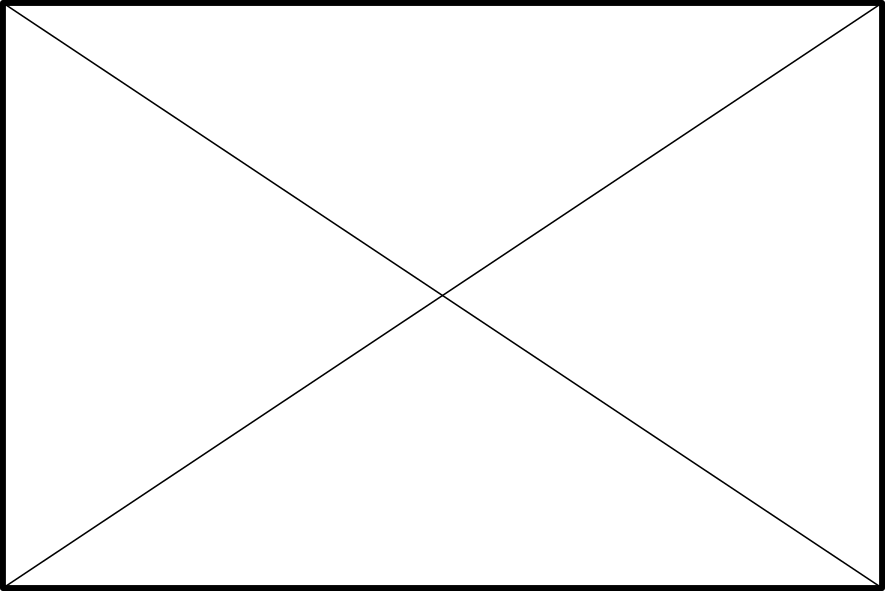
\includegraphics{TODO.png}
  \caption{Потенциометр против энкодера. Ручки обычно продают отдельно от
  самих сенсоров, чтобы можно было подобрать нужный размер и дизайн.}
\end{figure}

Потенциометр вполне подойдёт для регулировки громкости, но управлять с его помощью настройкой частоты будет не очень удобно. Смотрите сами, нам нужно выбирать частоту в диапазоне от 88.0 до 108.0 МГц с шагом 0.1. Всего получается 200 вариантов. При том что ручка типового потенциометры имеет ход в 270°. Выходит, что соседние станции могут разделять всего пара градусов поворота. Понадобится ювелирная настройка. Да, в природе существуют многооборотные потенциометры. Но они довольно редки и дороги. Более практичный выбор — поворотный энкодер в котором одно деление будет соответствовать одному шагу на 0.1 МГц.

Решено. В этом проекте мы воспользуемся обоими сенсорами: потенциометром для громкости и энкодером для подстройки частоты.

\section{Подключаем энкодер}

Энкодеры бывают разных типов. Они бывают импульсными или абсолютными. Абсолютные всегда знают в каком положении находятся, а импульсные лишь генерируют последовательности импульсов определённой формы, которые должен интерпретировать контроллер и сам рассчитывать угол поворота. Также энкодеры различаются по количеству выходов (2, 3, 4 и т.д.) и внутреннему устройству (магнитные, оптические, ёмкостные). У всех есть определённые достоинства и недостатки. Для нас важна доступность, поэтому будем использовать самый популярный в DIY-мире и простой \emph{квадратурный} импульсный энкодер.

Принцип работы такого энкодера изображён на рисунке \ref{fig:quadrature-encoder}. У него есть два выхода — A и B — каждый из которых может принимать значение логической единицы или нуля. Переключение значений происходит со смещением в полфазы относительно друг друга, поэтому всего на выходе возможны четыре комбинации значений. Отсюда и название: квадратурный.

\begin{figure}
  \centering
  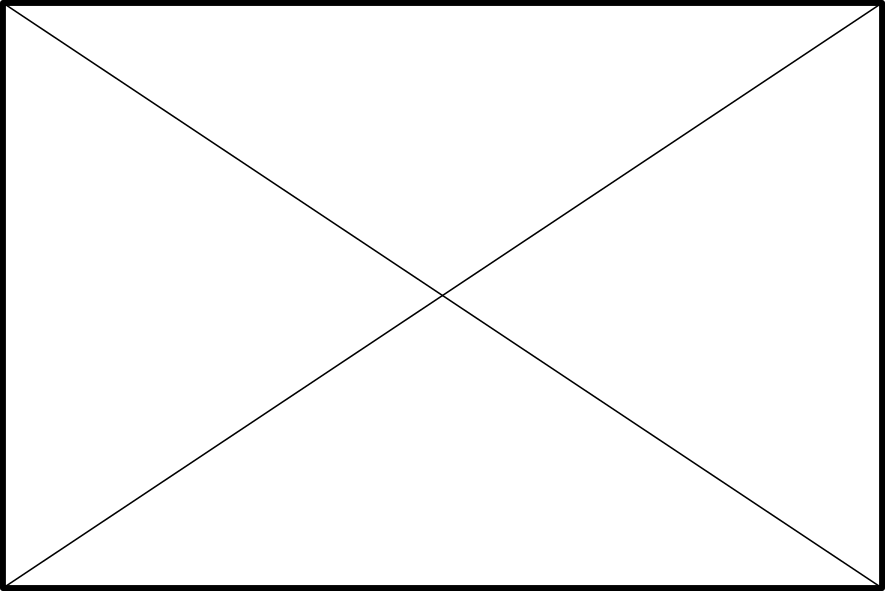
\includegraphics{TODO.png}
  \caption{Принцип работы импульсного квадратурного энкодера.}
  \label{fig:quadrature-encoder}
\end{figure}

Микроконтроллер должен фиксировать переключение сигналов A и B, и по изменению номера квадранта понимать, вращается ли ручка по часовой стрелке или против. В зависимости от этого можно либо наращивать внутренний виртуальный счётчик на один шаг, либо уменьшать.

Итак, чтобы задействовать наш энкодер для настройки радиоволны, подключите его к Arduino как показано на рисунке \ref{encoder-wiring}. В качестве пинов в нашем случае подойдут любые GPIO, которые не используются шиной I²C.\footnote{Для Arduino и Iskra Uno/Nano это A4 и A5; для Arduino и Iskra Leonardo/Neo/Micro это 2 и 3} Я выбрал пины 4 и 5.

\begin{figure}
  \centering
  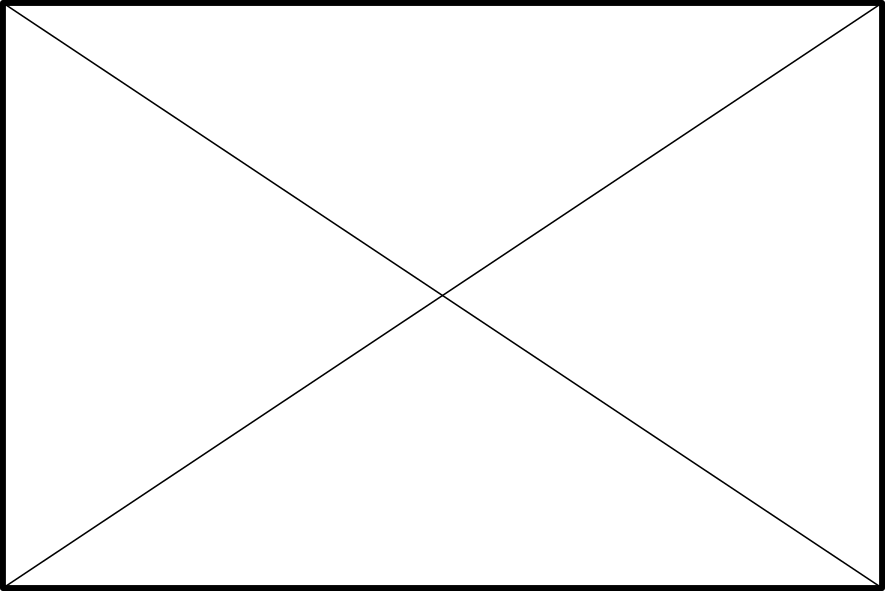
\includegraphics{TODO.png}
  \caption{Схема подключения энкодера к Arduino.}
  \label{encoder-wiring}
\end{figure}

В интернете можно встретить информацию о том, что подключать энкодер нужно строго к пинам, которые поддерживают так называемые аппаратные прерывания, но это обязательно только в тех устройствах, где переключения могут происходить очень быстро и есть шанс пропустить несколько переходов к очередной квадратуре из-за того, что контроллер был занят другой задачей. Например, это оправданно для подсчёта оборотов вала мотора. В нашем случае переключения происходят медленно, поэтому можно обойтись любыми цифровыми пинами.

\section{Ноды quad-encoder и count-bar}

Железо подключено, давайте программировать. Добавьте на свой патч ноду \texttt{quad-encoder} из \texttt{xod/common-hardware}. Её входы \texttt{PA} и \texttt{PB} определяют порты контроллера, куда подключен энкодер. Выставьте им значения \texttt{D4} и \texttt{D5} соответственно.

\begin{figure}
  \centering
  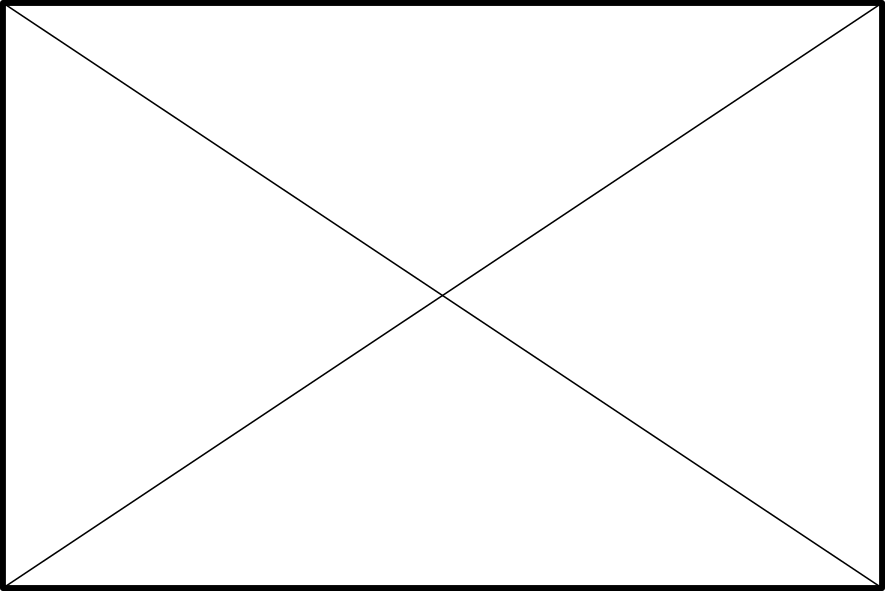
\includegraphics{TODO.png}
  \caption{Нода энкодера с отладочными вотчами на выходах.}
\end{figure}

У ноды есть два выхода: \texttt{INC} и \texttt{DEC}. Они генерируют пульсы при повороте на одно деление в одну или другую сторону соответственно. Проверьте сами, как это работает: подключите выходы к \texttt{xod/debug/watch-pulse}, загрузите программу на плату со включённой отладкой, поворачивайте ручку то в одну, то в другую сторону и наблюдайте, как увеличиваются счётчики пульсов.

Пульсы \texttt{INC} и \texttt{DEC} — это хорошо, но нам нужно управлять значением частоты в диапазоне от 88.0 до 108.0 с шагом 0.1. Как преобразовать пульсы в числовое значение? Специально для подобных случаев существует нода \texttt{count-bar} из стандартной библиотеки \texttt{xod/core}. Добавьте её на патч и рассмотрите входы:

\begin{itemize}
  \item \texttt{STEP} — цена деления, в нашем случае \texttt{0.1}, можно поставить отрицательное значение \texttt{-0.1}, если счёт идёт задом наперёд;
  \item \texttt{MIN}/\texttt{MAX} — предельные значения, в нашем случае \texttt{88.0} и \texttt{108.0} соответственно, счётчик будет оставаться на пределе при попытке выйти за диапазон;
  \item \texttt{INC}/\texttt{DEC} — пульс на увеличение/уменьшение значения на один шаг, возьмём эти пульсы с энкодера;
  \item \texttt{INIT} — начальное значение, пусть будет {88.0}.
\end{itemize}

Выход \texttt{OUT} содержит текущее накопленное значение и мы можем подать его непосредственно на вход ноде FM-приёмника. Финальный патч, вместе с отладочными нодами показан на рисинке \ref{patch:enc-count-freq}. Загрузите его на плату со включённой отладкой, крутите ручку и наблюдайте, как меняются значения. Не забудьте одеть наушники: радио уже как надо реагирует на свой первый орган управления!

\begin{figure}
  \centering
  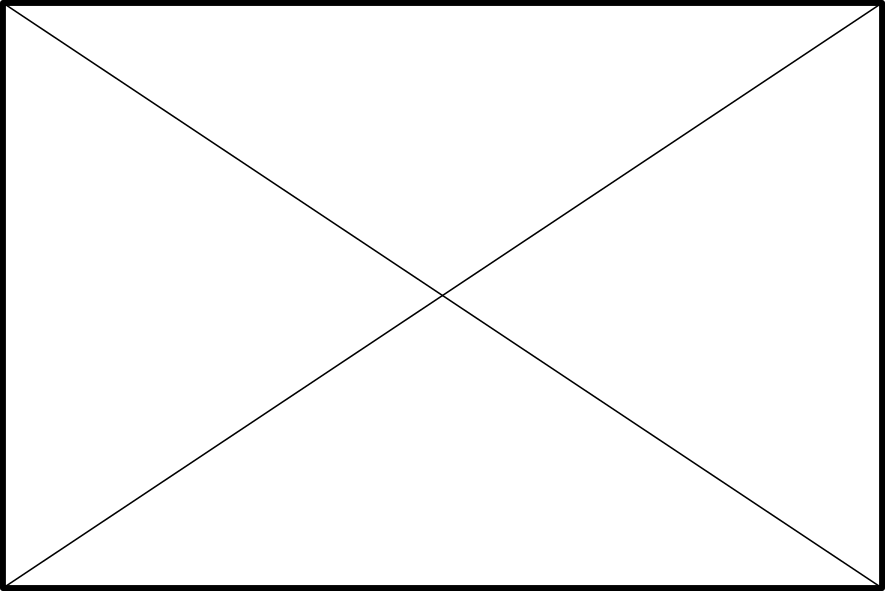
\includegraphics{TODO.png}
  \caption{Патч управления частотой радиостанции.}
  \label{patch:enc-count-freq}
\end{figure}
